\documentclass[11pt]{beamer}
\usetheme{Madrid}
\usefonttheme{serif}
\definecolor{customcolor}{RGB}{52,25,100} 
\setbeamercolor{structure}{fg=customcolor}

\usepackage[utf8]{inputenc}
\usepackage[T1]{fontenc}
\usepackage{amsmath}
\usepackage{amsfonts}
\usepackage{amssymb}
\usepackage{graphicx}
\usepackage{algorithm}
\usepackage{algpseudocode}
\usepackage{geometry}
\usepackage{hyperref}

\hypersetup{
    colorlinks=true,
    linkcolor=purple,
    filecolor=magenta,      
    urlcolor=cyan,
    pdftitle={Overleaf Example},
    pdfpagemode=FullScreen,
    }

\DeclareMathOperator{\sen}{sen}
\DeclareMathOperator{\tg}{tg}

\setbeamertemplate{caption}[numbered]

\newcommand{\decisionblock}[3]{
  \begin{block}{\textsc{#1}}
    \textbf{INSTANCE:} #2

    \vspace{0.8em}

    \textbf{QUESTION:} #3
  \end{block}
}

\author[Atishaya Maharjan]{\underline{Atishaya Maharjan}, Stephane Durocher, Jimmy Zhu}
\title{Geometric Spanning Trees that Minimizes the Wiener Index}
\newcommand{\email}{maharjaa@umanitoba.ca}
\setbeamertemplate{navigation symbols}{} 
\institute[]{University of Manitoba\par Geometric, Approximation, and Distributed Algorithms (GADA) lab} 
\date{\today} 

\bibliographystyle{apalike}

\begin{document}

\begin{frame}
	\titlepage
\end{frame}

\begin{frame}{Wiener Index in Graphs}
	\begin{itemize}
		\item Let $G = (V, E)$ be a weighted undirected graph and let $\delta_G(u, v)$ denote the \textbf{shortest (minimum-weight) path}  between vertices $u$ and $v$ in $G$.
		      \pause
		\item The Wiener index is defined as:
		      \[
			      W(G) = \sum_{u, v \in V} \delta_G(u, v)
		      \]
		      \pause
	\end{itemize}
	\begin{center}
		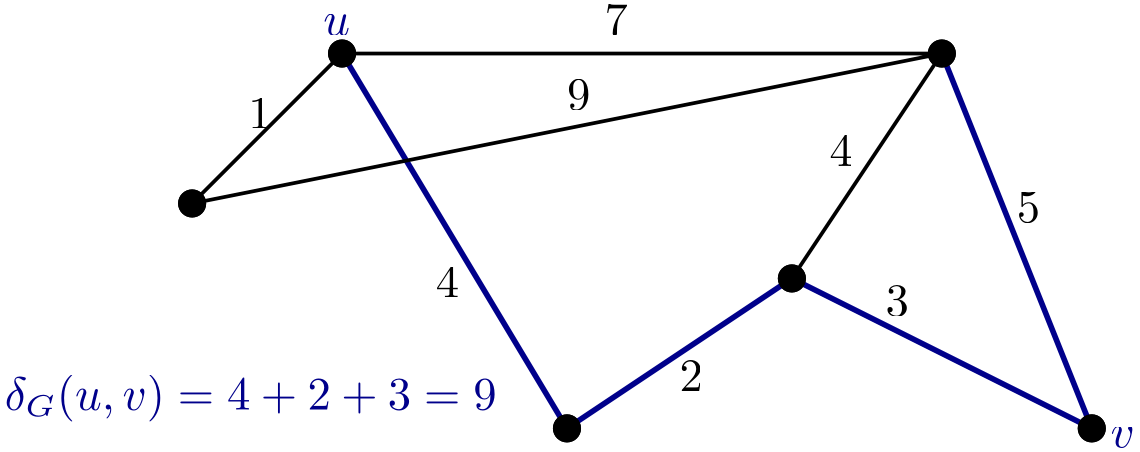
\includegraphics[width=0.75\textwidth]{images/wiener_index.png} % Replace with your own
	\end{center}
\end{frame}

\begin{frame}{Wiener Index in Network Design}
	\begin{itemize}
		\item Given an undirected graph $G = (V, E)$ and a non-negative weight function $w: E \to \mathbb{R}^+$, the goal is to find a spanning tree $T$ of $G$ that minimizes the Wiener index.
		      \pause
		\item The \textbf{routing cost} $c(T)$ of a spanning tree $T$ of $G$ is:
		      \[
			      c(T) = \sum_{u, v \in V} \delta_T(u, v)
		      \]
		      \pause
	\end{itemize}

	\begin{block}{The Minimum Routing Cost Spanning Tree (MRCST) problem}
		\begin{itemize}
			\item Input: A graph $G = (V, E)$ with a non-negative weight function $w: E \to \mathbb{R}^+$.
			\item Output: A spanning tree $T$ of $G$ that minimizes the routing cost $c(T)$.
		\end{itemize}
	\end{block}
	\begin{itemize}
		\pause
		\item The MRCST problem is NP-Complete. There exists a PTAS for MRCST.
	\end{itemize}
\end{frame}

\begin{frame}{Problem Statement: Geometric Spanning Trees}
	\textbf{Reference:} WADS 2023 ~\cite{article:geometric_spanning_trees_minimizing_wiener_index}

	\begin{enumerate}
		\item Input: A set $P$ of $n$ points in the plane.
		\item Goal: Construct a \textbf{spanning tree} on $P$ that minimizes the \textbf{Wiener index}.
		\item The weight function is defined as the Euclidean distance between points.
	\end{enumerate}
\end{frame}

\begin{frame}{Results Summary: Geometric Spanning Trees}
	\begin{itemize}
		\item Spanning tree of $P$ that minimizes the Wiener index is planar.
		      \pause
		\item When $P$ is in convex position, this can be solved in polynomial time.
		      \pause
		\item The hamiltonian path of $P$ that minimizes the Wiener index is not necessarily planar.
		      \pause
		\item Computing such a hamiltonian path is NP-Hard.
		      \pause
		\item There exists a $(1 + \varepsilon)-$Approximation algorithm for finding a Hamiltonian path that minimizes the Wiener index.*
	\end{itemize}

	* This relies on distortion embeddings and is overall complicated to implement.
\end{frame}

\begin{frame}{Divide and Conquer Algorithm for Approximating Hamiltonian Paths}
	\begin{algorithm}[H]
		\caption{DivideAndConquerWiener($P$)}
		\begin{algorithmic}[1]
			\Procedure{DivideAndConquerWiener}{$P$, $depth = 0$, $maxDepth = 10$}
			\If{$|P| \leq 4$ or $depth > maxDepth$}
			\State \Return \Call{BruteForceHamiltonianPath}{$P$}
			\EndIf
			\State $(a, b, c) \gets$ \Call{FindMidpointLine}{$P$}
			\State $(P_L, P_R) \gets$ \Call{PartitionPoints}{$P$, $a$, $b$, $c$}
			\State $\pi_L \gets$ \Call{DivideAndConquerWiener}{$P_L$, $depth+1$}
			\State $\pi_R \gets$ \Call{DivideAndConquerWiener}{$P_R$, $depth+1$}
			\State \Return \Call{OptimalConnectPaths}{$\pi_L$, $\pi_R$}
			\EndProcedure
		\end{algorithmic}
	\end{algorithm}
\end{frame}

\begin{frame}{Divide and Conquer Algorithm for Approximating Hamiltonian Paths}
	Analyzing DivideAndConquerWiener proved to be very difficult. Initially, I thought it was a $\mathcal{O}(\log(n))$-Approximation but I could not show it.

	I did additional empirical experiments with Python which you can find it here: \href{https://github.com/Atishaya7777/spatially_embedded_graph/tree/main/scripts}{github.com/Atishaya7777/spatially\_embedded\_graph}
\end{frame}

\begin{frame}{Hardness Proof}
	\begin{decisionblock}{Euclidean Wiener Index Tree Problem (EWITP)}
		{A set $P$ of $n$ points in $\mathbb{R}^2$, a cost $W$, and a budget $B$.}
		{Does there exist a spanning tree $T$ of $P$ such that $W(T) \leq T$ and $wt(T) \leq B$?}
	\end{decisionblock}

	Here, $W(T)$ denotes the Wiener index of the tree $T$ and $wt(T)$ denotes the total weight of the tree $T$.

	\begin{decisionblock}{Partition}
		{A set $X = \{x_1, x_2, \dots, x_n\}$, where $x_i \in \mathbb{Z}$ such that $R = \displaystyle\sum_{i = 1}^{n}x_i$.}
		{Does there exists a subset $S \subseteq X$ such that $\displaystyle\sum_{x_i \in S}x_i = \dfrac{R}{2}$.}
	\end{decisionblock}
\end{frame}

\begin{frame}{Hardness Proof}
	The following reduction is from \cite{article:geometric_spanning_trees_minimizing_wiener_index}.
	\begin{definition}
		Let $P$ be a set of $n$ points in $\mathbb{R}^2$ and let $T$ be a spanning tree of $P$.
		For an edge $(p, q) \in T$, we define $N_T(p, q) = |\{x\in P: \delta_T(p, x) < \delta_T(q,x)\}|$ be the number of points in $T$ that are closer to $p$ than to $q$.
	\end{definition}
\end{frame}

\begin{frame}{Hardness Proof}
	Given an instance $X = \{x_1, x_2, \dots, x_n\}$ of the \textbf{PARTITION} instance where $x_i \in \mathbb{Z}$:
	\begin{itemize}
		\item Construct a set $P$ of $m = n^3 + 3n + 1$ points.
		      \begin{itemize}
			      \item A point $s$ and $n$ points $p_1, p_2, \dots p_n$ located equally spaced on a circle of radius $nR$ centered at $s$.
			      \item A cluster $C$ of $n^3$ points located at the center of the circle of radius $\dfrac{1}{n^{10}R}$ centered at $S$.
			      \item For each $1 \leq i \leq n$, we have two points $l_i$ and $r_i$ both of distance $x_i$ from $p_i$ and the distance between them is $\dfrac{x_i}{2}$.
		      \end{itemize}
		\item Set
		      \begin{align*}
			      B & = \left(n^2 + \dfrac{7}{4}\right)R + \dfrac{1}{n^7R}                                             \\
			      W & = 3n^2(m - 3)R + \left(\dfrac{9}{4}m - \dfrac{13}{4}\right)R + \dfrac{1}{n^4R} + \dfrac{3}{n^6R} \\
			        & = 3n^5R + \dfrac{45}{4}n^3R - 6n^2R + \dfrac{27}{4}nR - R + \dfrac{1}{n^4R} + \dfrac{3}{n^6R}
		      \end{align*}
	\end{itemize}
\end{frame}

\begin{frame}{Hardness Proof}
	\begin{figure}
		\centering
		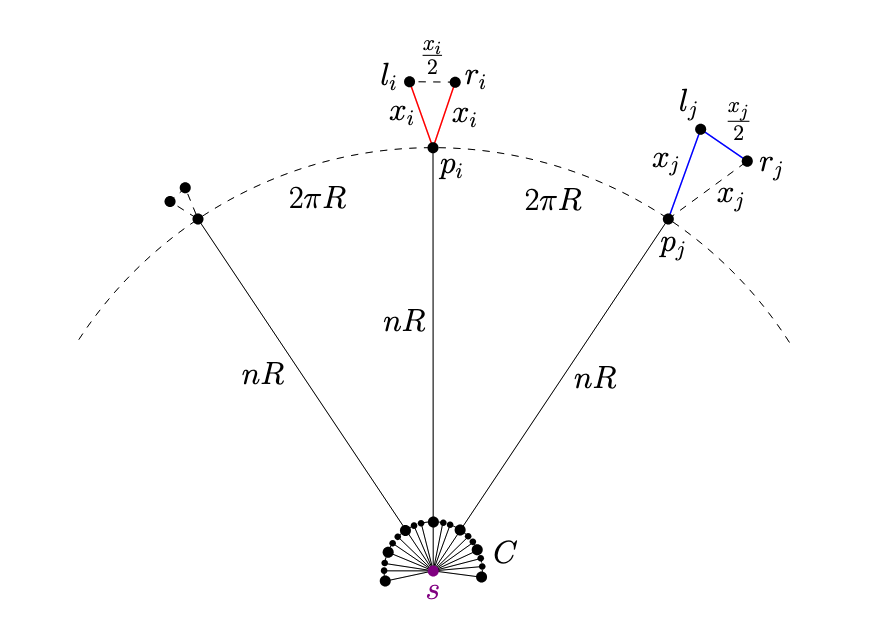
\includegraphics[width=0.7\textwidth]{images/construction.png}
		\caption{The set $P$ produced by the reduction. Connecting the points $l_j, r_j$, and $p_j$ for $x_j \in S$ (Blue) and connecting the points $l_i, r_i$, and $p_i$ for $x_i \in X \setminus S$ (Red).}
	\end{figure}
\end{frame}

\begin{frame}{Hardness Proof}
	Assume there exists a set $S \subseteq X$ such that $\displaystyle\sum_{x_i \in S}^{x_i} = \dfrac{R}{2}$.

	Construct a spanning tree $T$ for the points of $P$ as follows:
	\begin{itemize}
		\item $E_1 = \{(s, p_i): 1 \leq i\leq n\}$
		\item $E_2 = \{(p_i, l_j), (p_i, r_i): x_i \in S\}$
		\item $E_3 = \{(p_j, l_j), (l_j, r_j): x_j \in X \setminus S\}$, and
		\item $E_4 = \{(s, p): p \in C\}$
	\end{itemize}
\end{frame}

\begin{frame}{Weight of the Tree}
	\begin{align*}
		wt(T) & = wt(E_1) + wt(E_2) + wt(E_3) + wt(E_4)                  \\
		      & = n^2R + R + \dfrac{3}{4}R + n^3\cdot \dfrac{1}{n^{10}R} \\
		      & = \left(n^2 + \dfrac{7}{4}\right)R + \dfrac{1}{n^7R}     \\
		      & = B
	\end{align*}
\end{frame}

\begin{frame}{Wiener Index of the Tree}
	\begin{align*}
		W(T) & = \displaystyle\sum_{(p, q) \in T} N_T(p, q) \cdot N_T(q, p) \cdot |pq|        \\
		     & = \displaystyle\sum_{(p, q) \in E_1} N_T(p, q) \cdot N_T(q, p) \cdot |pq|      \\
		     & \quad+ \displaystyle\sum_{(p, q) \in E_2} N_T(p, q) \cdot N_T(q, p) \cdot |pq| \\
		     & \quad+ \displaystyle\sum_{(p, q) \in E_3} N_T(p, q) \cdot N_T(q, p) \cdot |pq| \\
		     & \quad+ \displaystyle\sum_{(p, q) \in E_4} N_T(p, q) \cdot N_T(q, p) \cdot |pq| \\
		     & = W (\text{Chalk \& Talk})
	\end{align*}
\end{frame}

\begin{frame}{Converse direction}
	It is a matter of computation to show that:
	\begin{theorem}[Claim 4]
		There are exactly $n$ edges in $T$ between the points in $C \cup \{s\}$ and the others.
	\end{theorem}

	The paper shows it considering the cases of there are more than $n$ edges and less than $n$ edges and shows a contradiction.
\end{frame}

\begin{frame}{Converse direction}
	Let $P_i$ denote the triplet $\{p_i, l_i, r_i\}$ for $1 \leq i \leq n$.
	\begin{itemize}
		\item From Claim 4, it follows that for every $1 \leq i \leq n$, there is exactly one edge $(p, q)$ in $T$ for which $p \in C \cup \{s\}$ and $q \in P_i$. Note that $q = p_i$.
		\item Thus, in every $P_i$, we have $(p_i, l_i) \in T$ or $(p_i, r_i) \in T$.
		\item WLOG let $(p_i, l_i) \in T$:
		      \begin{itemize}
			      \item Either $(p_i, r_i) \in T$ OR $(l_i, r_i) \in T$.
			      \item Let $S \subseteq X$ such that $x_i \in S \iff (p_i, r_i) \in T$.
			      \item Let $R' = \displaystyle\sum_{x_i \in S}x_i$.
		      \end{itemize}
	\end{itemize}

	They then argue that if $R' \neq \dfrac{R}{2}$, then either $wt(T) > B$ or $W(T) > W$.

	\vspace{0.5em}

	\begin{center}
		\textbf{This concludes the hardness result.}
	\end{center}
\end{frame}

\begin{frame}{Why is the bound $wt(T) \leq B$ important?}
	The weight bound is what forces the gadgets to connect in a very specific way (open or closed), which in turn encodes the binary choices in \textbf{PARTITION}.

	\begin{itemize}
		\item $n$ gadgest for each integer $x_i \in X$, giving two connection options:
		      \begin{itemize}
			      \item \textbf{Open}: $(p_i, l_i)$ and $(p_i, r_i)$ contributing $2x_i$ weight.
			      \item \textbf{Closed}: $(p_i, l_i)$ and $(l_i, r_i)$ contributing $\frac{3x_i}{2}$ weight.
		      \end{itemize}
	\end{itemize}

	If we takeout the weight bound:
	\begin{itemize}
		\item We could just have everything open, which might reduce the Wiener index (Since open gadgets keep gadget paths short), but increase the weight
		\item In the unbounded case, we would have no reason to avoid such trees.
	\end{itemize}
\end{frame}

\begin{frame}{Next Steps and Open Problems?}
	\begin{itemize}
		\item Preliminarily, I think the modification to the reduction needs to happen such that the penalty is no longer on the weight but solely on the Wiener Index. Of course, this is harder to prove.
		\item Primiarly, construct gadgets so that the only correct combination of open/closed configurations minimize the Wiener Index.
	\end{itemize}
\end{frame}

\begin{frame}[allowframebreaks]{References}
	\bibliography{references}
\end{frame}

\begin{frame}
	\begin{center}
		The end.

		\email
	\end{center}
\end{frame}

\end{document}
